\documentclass{article}
\usepackage{graphicx}

\begin{document}

\section{Gráfico}

A continuación se muestra el gráfico generado:

\begin{figure}[h]
    \centering
    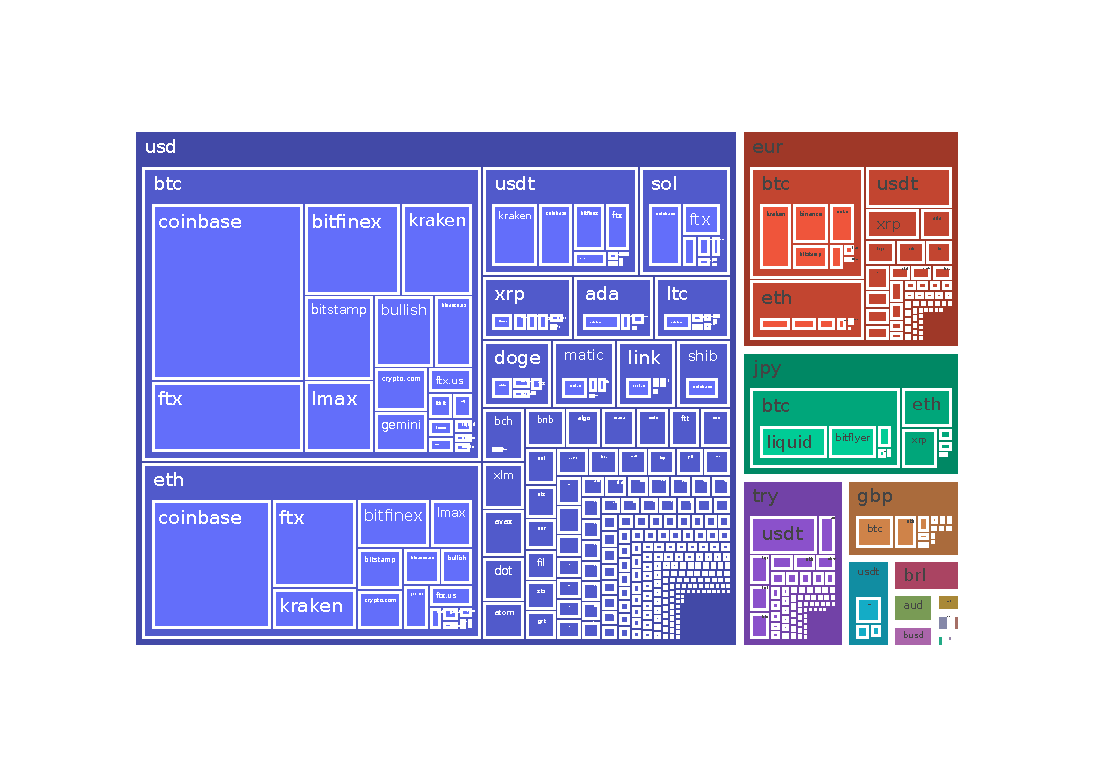
\includegraphics[width=0.8\textwidth]{grafico.pdf} % Asegúrate de tener un archivo grafico.pdf en la misma carpeta o especifica la ruta correcta
    \caption{Gráfico generado con Plotly}
    \label{fig:grafico}
\end{figure}

\end{document}